\documentclass[
	%sans,			% use sans-serif font
	%serif,			% use serif-font
	%mathsans,		% set mathtext to sans-serif
	%mathserif,		% set mathtext to serif
	%10pt,
	10pt,
	%12pt,
	t		% add text at the top border of slide
	%slidescentered,% center text on slide
	%draft,			% compile as draft version
	%handout,		% create handout file
	%notes,			% include nodes in slides
	%compress		% compress navigation bar
]{beamer}

\usetheme{lmtslides}
\usepackage{eso-pic}
\usepackage{graphicx}
%\usepackage[pdftex]{color}
\usepackage{times}
\usepackage[latin1]{inputenc}
%\usepackage[T1]{fontenc}
\usepackage[amssymb]{SIunits}
\usepackage{amsmath,amssymb}
\usepackage{eurosym}
\usepackage{booktabs}
\usepackage{colortbl}
\usepackage{url}
\usepackage[absolute,overlay]{textpos}
\usepackage{graphicx}
\usepackage{mathtools}
\usepackage{pifont}% http://ctan.org/pkg/pifont
\usepackage{appendixnumberbeamer}
\usepackage{subcaption}

\newcommand{\xmark}{\ding{55}}%
\newcommand{\cmark}{\ding{51}}%

\renewcommand{\footnoterule}{\vfill\kern -3pt  \kern 2.6pt}

\setbeamertemplate{caption}{\raggedright\insertcaption\par}
\setbeamertemplate{bibliography item}[online]
\graphicspath{{figures/}}

\setlang{en}		

% Supervisor: Univ.-Prof. Dr. Hans-Joachim Bungartz
% Advisors: Manish Kumar Mishra, M.Sc. (hons) &
% Samuel James Newcome, M.Sc.

% MODIFY THESE ACCORDINGLY! ---
\title{Algorithm Selection and Auto-Tuning in AutoPas}
\type{Sf} % (M/B/D/S)(f/m): (Master/Bachelor/Diplom/Studienarbeit)(final/midterm)
\author{Manuel Lerchner}
\email{manuel.lerchner@tum.de}
\advisorOne{Manish Kumar Mishra, M.Sc. (hons)}
\date{\today}
%------------------------------



\AtBeginSection[]
{
    \begin{frame}
        \frametitle{Table of Contents}
        \tableofcontents[currentsection,currentsubsection]
    \end{frame}
}

%%%%%%%%%%%%%%%%%%%%%%%%%%
\begin{document}

\maketitle

\setcounter{framenumber}{0}

\section{Introduction}
\begin{frame}
    \frametitle{What is AutoPas?}

    \begin{textblock*}{5cm}(9cm,1.8cm)
        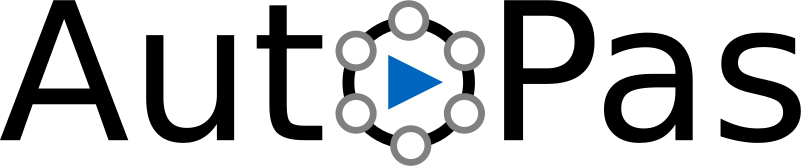
\includegraphics[width=3cm]{figures/AutoPasLogo}
    \end{textblock*}

    \begin{itemize}
        \item Library for arbitrary N-body simulations
        \item Optimal performance by switching implementations
              \begin{itemize}
                  \item \textbf{Container:} Finding neighboring particles
                  \item \textbf{Traversal:} Parallel force calculations
                  \item \textbf{Data Layout:} Memory access optimization
                  \item \textbf{Newton 3:} Force calculation optimization
              \end{itemize}
    \end{itemize}

    \vspace{-0.1cm}
    \begin{figure}
        \centering
        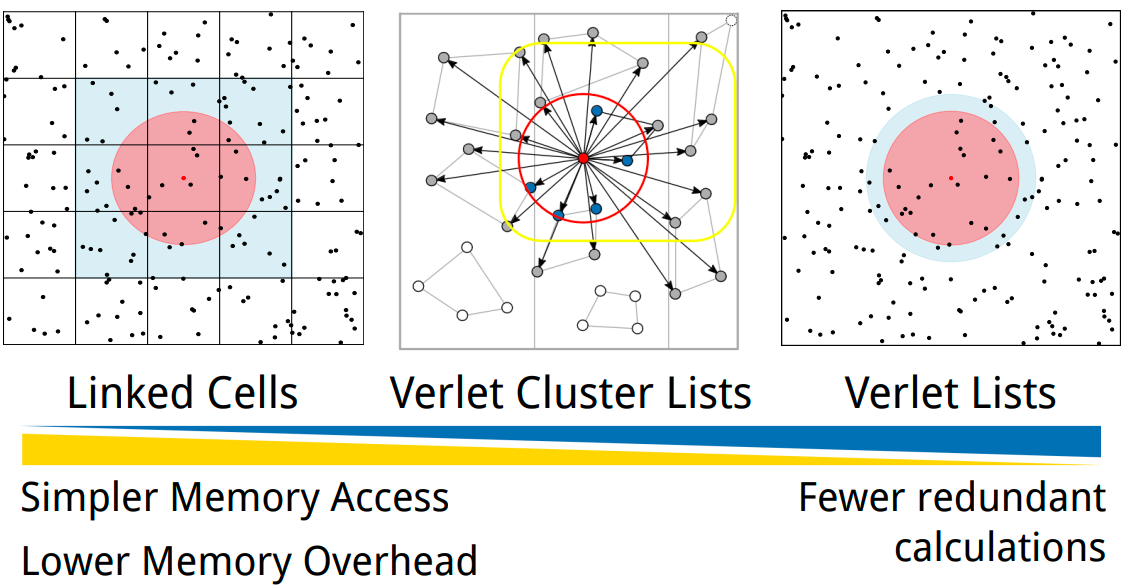
\includegraphics[width=0.72\textwidth]{figures/traversals.png}
    \end{figure}

    \begin{textblock*}{5cm}(6.3cm,9.35cm)
        \tiny{\cite{SIAM_PP24}}
    \end{textblock*}

\end{frame}


\begin{frame}
    \frametitle{Structure of AutoPas}

    \begin{itemize}
        \item Three main areas:
              \begin{itemize}
                  \item User Application
                  \item Algorithm Library
                  \item Tuning Strategies
              \end{itemize}
        \item Algorithm Library:
              \begin{itemize}
                  \item Huge Search Space\footnote{\scriptsize{$\text{Container}\times\text{Traversal} \times \text{Data Layout} \times \text{Newton 3} \times \text{Load Estimator} \times \text{Cell Size Factor}$}
                        }
              \end{itemize}
        \item Tuning Strategies:
              \begin{itemize}
                  \item Full Search
                  \item Random Search
                  \item Predictive Tuning
                  \item Bayesian Search
                  \item Rule Based Tuning
              \end{itemize}
    \end{itemize}

    \begin{textblock*}{4cm}(8cm,2cm)
        \begin{figure}
            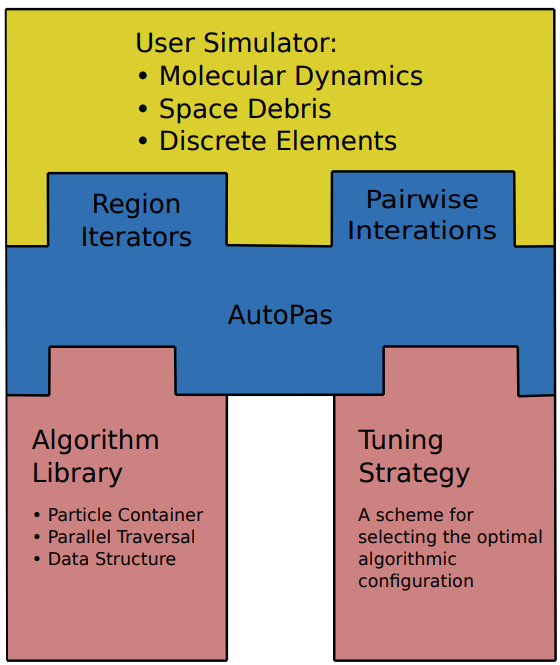
\includegraphics[width=4cm]{figures/AutoPasLibraryStructure.png}
            \caption{ \scriptsize{\cite{Newcome2023Poster}}}

        \end{figure}
    \end{textblock*}
\end{frame}



\begin{frame}
    \begin{center}
        \vspace{1cm}
        {\large \textbf{Thank you for your attention!}}

        \vspace{2cm}

        \Huge{Questions?}
    \end{center}
\end{frame}

\begin{frame}[allowframebreaks, noframenumbering]
    \frametitle{References}
    \footnotesize
    \bibliographystyle{apalike}
    \bibliography{literature}
\end{frame}

\appendix

\begin{frame}
    \frametitle{Backup:}

    \begin{itemize}
        \item A
        \item B
    \end{itemize}
\end{frame}



\end{document}